\documentclass[runningheads]{llncs}
\usepackage[T1]{fontenc}
\usepackage{graphicx}
\usepackage{float}
\usepackage{amsmath,amssymb}
\usepackage{booktabs}
\usepackage{multirow}
\usepackage{xcolor}
\usepackage{microtype}
\usepackage{enumitem}
\usepackage{hyperref}
\renewcommand\UrlFont{\color{blue}\rmfamily}
\urlstyle{rm}
\raggedbottom
\AtBeginDocument{
  \setlength{\abovedisplayskip}{4pt}
  \setlength{\belowdisplayskip}{4pt}
  \setlength{\abovedisplayshortskip}{0pt}
  \setlength{\belowdisplayshortskip}{0pt}
}
\graphicspath{{figures/}}
\begin{document}
\title{Feature Geometry Does Not Predict Segmentation Quality:\texorpdfstring{\\}{ }Spatial Autocorrelation as a Label-Free Diagnostic for Frozen ViTs}
\titlerunning{Feature Geometry Does Not Predict Segmentation Quality}
\author{Thai Quang Tran\inst{1}\orcidID{0009-0000-4674-4388} \and
Nguyen Tan Khoi Nguyen\inst{1}\orcidID{0009-0009-7970-9883} \and
Phuoc Tan Phan\inst{1}\orcidID{0009-0003-7078-9406} \and
Khai Tien Trinh\inst{1}\orcidID{0009-0002-0447-5743}}
\authorrunning{T.\,Q. Tran et al.}
\institute{FPT University, Ho Chi Minh Campus, Vietnam\\
\email{\{tranquangthai1029, nguyennguyentankhoi,
phanphuoc9113, khaitrinh2005\}@gmail.com}}
\maketitle

% ============================================================
% ABSTRACT
% ============================================================
\begin{abstract}
Can we predict how well a frozen ViT backbone will segment images, without labels? We evaluate eight metrics on eleven self-supervised ViT-B/16 backbones and find that \emph{every} feature-geometry metric fails to predict segmentation quality---including local intrinsic dimensionality, which rules out ``global vs.\ local'' as the relevant distinction. Only Patch Spatial Autocorrelation (PSA)---which measures how smoothly features vary across neighboring patches---significantly predicts Segmentation Covering across BSDS500 ($r=0.862$), COCO ($r=0.876$), and ADE20K ($r=0.833$), robust across all leave-one-out subsets. Extended evaluation on 16 models reveals when PSA breaks down: models trained with contextualized reconstruction (Data2Vec) or multimodal alignment (BEiT3) inflate PSA without preserving local spatial semantics. For backbone selection in dense prediction, the right question is not \emph{how rich} the features are, but \emph{how spatially coherent} they are.
\keywords{Self-supervised learning \and Vision Transformer \and unsupervised segmentation \and spatial autocorrelation \and backbone selection \and representation quality.}
\end{abstract}

% ============================================================
% 1. INTRODUCTION
% ============================================================
\section{Introduction}

Self-supervised Vision Transformers (ViTs) are the default feature extractors for unsupervised segmentation. Frozen features from models trained via self-distillation \cite{caron2021}, masked autoencoding \cite{he2022}, or contrastive alignment \cite{radford2021} are widely used for dense prediction via clustering \cite{hamilton2022,curie2025}, spectral decomposition \cite{melas2022,kim2024eagle}, and graph partitioning \cite{couairon2024diffcut}. A practical question follows: \textit{how can we select the best backbone for a dense prediction task without labeled data?}

Eigenspectral metrics like RankMe \cite{garrido2023} predict classification accuracy from the singular value distribution, but they were designed and validated exclusively on classification tasks. Recent work has shown that SSL evaluation protocols do not transfer reliably across downstream tasks \cite{ijcv2025ssl}---a model ranked highly for classification may perform poorly on segmentation, and vice versa. Current unsupervised segmentation methods such as EAGLE \cite{kim2024eagle} and DiffCut \cite{couairon2024diffcut} select backbones empirically via labeled validation; as these pipelines scale to label-scarce domains, eigenspectral metrics are the only available proxy---yet have never been systematically tested for dense prediction.

We fill this gap with an evaluation of eight metrics across eleven frozen self-supervised ViT-B/16 backbones, organized into two classes: \emph{feature geometry} metrics that characterize the representation space (whether globally or locally), and \emph{spatial arrangement} metrics that measure patch-level structure in image or attention space. Among the latter, Patch Spatial Autocorrelation (PSA)---the mean cosine similarity between each patch feature and its spatial neighbors---emerges as the only significant predictor.

Our main contributions are: (1)~\textbf{Categorical Failure of Feature Geometry}: all four feature geometry metrics, including LID (a local metric), fail to predict segmentation quality ($r \leq -0.38$, all $p > 0.13$), ruling out ``global vs.\ local'' as the relevant distinction (Sect.~\ref{sec:metric_taxonomy}); (2)~\textbf{PSA as Significant Predictor}: only PSA significantly correlates with SC ($r=0.862$, $p=0.0007$, $N=11$, stable across all leave-one-out subsets), and its correlation is not tautological---three other spatial-domain metrics fail (Sect.~\ref{sec:results}); (3)~\textbf{Cross-Dataset Generalization}: PSA predicts SC on BSDS500, COCO ($r=0.876$, $p=0.0004$), and ADE20K ($r=0.833$, $p=0.0015$) when architecture is controlled (Sect.~\ref{sec:boundary}); (4)~\textbf{Mechanistic Boundary Conditions}: extending to 16 models maps where PSA fails---contextualized reconstruction (Data2Vec) and multimodal alignment (BEiT3) inflate PSA without preserving semantic boundaries (Sect.~\ref{sec:boundary_conditions}); (5)~\textbf{Dual-Level Spectral Failure}: spectral complexity predicts worse SC both across backbones ($r=-0.43$) and within individual backbones (4 of 6 at $p<0.01$), but for different reasons---pretraining paradigm vs.\ scene clutter (Sect.~\ref{sec:simpson}).

% ============================================================
% 2. RELATED WORK
% ============================================================
\section{Related Work}

\subsection{Self-Supervised Features for Segmentation}
Frozen features from self-supervised ViTs---including DINO/DINOv2 \cite{caron2021,oquab2024}, MAE \cite{he2022}, CLIP \cite{radford2021}, and MoCo-v3 \cite{chen2021mocov3}---are widely used for segmentation via clustering \cite{wang2023lightweight,amir2022}, spectral methods \cite{melas2022,kim2024eagle,couairon2024diffcut}, and learned refinement \cite{hamilton2022,curie2025}. The literature implicitly assumes that backbone choice determines quality \cite{amir2022}; we test whether that quality can be predicted without labels, and whether rankings depend on the clustering algorithm's geometric assumptions.

\subsection{Representation Quality Metrics}
RankMe \cite{garrido2023} and $\alpha$-ReQ \cite{agrawal2022} assess quality via eigenspectral properties. RankMe predicts classification accuracy without labels via the Shannon entropy of singular values. While RankMe is unreliable across diverse model families even for ImageNet \cite{tsitsulin2023}, existing validations target global representations; whether these metrics predict dense pixel-level segmentation quality \cite{ijcv2025ssl} remains untested. We provide the first systematic evaluation covering both global and local geometry metrics alongside spatial arrangement metrics---a distinction the literature has not drawn.

\subsection{Alignment, Uniformity, and Feature Complementarity}
Feature quality decomposes into alignment and uniformity \cite{wang2020alignment,bardes2022vicreg}---paralleling semantic coherence and spectral diversity. The complementarity between CLIP's semantic alignment and DINO's spatial precision is well-documented \cite{tong2024eyes,wysoczanska2024clipdinoiser}. This motivates our cross-dataset analysis (Sect.~\ref{sec:boundary}), where backbone rankings reverse across annotation granularity---a reversal that no eigenspectral metric tracks.

% ============================================================
% 3. METHODOLOGY
% ============================================================
\section{Methodology}

We use a minimal pipeline---eschewing learnable decoders or heavy post-processing---to ensure that segmentation differences strictly reflect intrinsic feature quality. Given an input image $I \in \mathbb{R}^{H \times W \times 3}$, a frozen ViT extracts patch tokens at stride $p$, which are bilinearly upsampled to pixel resolution, $\ell_2$-normalized, and reduced to $d\!=\!32$ dimensions via PCA. Performance saturates at $d\!=\!32$ ($\text{SC} \approx 0.58$); sweeping $d \in \{8, 16, 32, 48, 64, 128\}$ confirms this preserves spectral richness while filtering noise. Features are then partitioned into $K\!=\!4$ clusters via K-Means; SC peaks at $K\!=\!4$ and drops monotonically for $K \geq 5$ (ablation: $K\!=\!2{:}0.557$, $K\!=\!4{:}0.579$, $K\!=\!10{:}0.468$ on BSDS500 with DINO ViT-S/8). We additionally report Boundary F1-score (BF1) to verify rankings are not artifacts of $K$-sensitivity. The full pipeline is illustrated in Fig.~\ref{fig:pipeline}.

\begin{figure}[H]
    \centering
    \includegraphics[width=\textwidth]{generated.png}
    \caption{Pipeline overview. Frozen ViT features are upsampled, normalized, and clustered. Class~A metrics ($n_{80}$, LID, NESum, Stable~Rank) are computed from raw features via SVD; Class~B metrics include PSA (from PCA features) and attention-based metrics (AttnGap, AttnEntropy, AttnPR) from the ViT backbone.}
    \label{fig:pipeline}
    \vspace{-15pt}
\end{figure}

\subsection{Backbones and Clustering Algorithms}
\label{sec:backbones}

We evaluate sixteen ViT backbones spanning multiple pre-training paradigms. To isolate pre-training paradigm from architectural capacity, our core metric evaluations (Sect.~\ref{sec:results}) use a \emph{controlled SSL set} of eleven self-supervised ViT-B/16 models (86M parameters, patch size 16): DINO, MAE, CLIP, SigLIP, MoCo-v3, BEiT, BEiTv2, iBOT, EVA-02, OpenCLIP (LAION-2B), and MetaCLIP (2.5B). EVA-02 combines CLIP and masked image modeling; OpenCLIP and MetaCLIP probe the effect of training data scale and curation on contrastive features. To establish boundary conditions (Sect.~\ref{sec:boundary_conditions}), we additionally evaluate five out-of-distribution models: supervised baselines (DeiT, DeiT-III), a segmentation-supervised oracle (SAM), and two mechanistic outliers (Data2Vec for contextualized latent reconstruction, BEiT3 for multimodal alignment). For clustering-invariant and cross-dataset analyses (Sects.~\ref{sec:clustering},~\ref{sec:boundary}), we add DINO ViT-S/8 and DINOv2 ViT-S/14 (22M parameters) to form a \emph{mixed-architecture set}. Most SSL models are pre-trained on ImageNet-1K; exceptions are CLIP (WIT-400M), SigLIP (WebLI-12B), OpenCLIP (LAION-2B), MetaCLIP (2.5B), EVA-02 (Merged-2B), and DINOv2 (LVD-142M). DINO ViT-B/16 uses the official \texttt{dino\_vitb16} checkpoint from \texttt{facebookresearch/dino}.

We test three clustering algorithms: \textbf{K-Means} (spherical clusters via cosine similarity after $\ell_2$-normalization); \textbf{GMM} (full-covariance elliptical clusters on the 32-d PCA subspace); and \textbf{Spectral Clustering} (affinity-based partitioning on a 5{,}000-pixel subsample, assuming only local manifold connectivity).

\subsection{Metric Taxonomy}
\label{sec:metric_taxonomy}

We organize candidate metrics into two classes based on what they measure.

\paragraph{Class A: Feature Geometry.} Given the pixel-feature matrix $F \in \mathbb{R}^{N \times D}$, we compute singular values $\{\sigma_i\}$ and eigenvalues $\lambda_i = \sigma_i^2 / (N-1)$. RankMe \cite{garrido2023} measures effective rank via Shannon entropy of singular values; it is highly correlated with $n_{80}$ ($r > 0.95$ across our backbones), so we report $n_{80}$ as representative. The four Class A metrics are: \textbf{$n_{80}$}, a global metric tracking the minimum components needed for 80\% variance; \textbf{NESum} and \textbf{Stable Rank}, which measure global spectral spread via normalized eigenvalue sum $\sum_i \sigma_i / \sigma_1$ and ratio $\sum_i \sigma_i^2 / \sigma_1^2$ respectively; and \textbf{LID}, a local metric measuring intrinsic manifold dimensionality around each patch feature via the Method of Moments \cite{amsaleg2018lid}.

\paragraph{Class B: Spatial Arrangement.} The four Class B metrics are: \textbf{PSA}, the mean cosine similarity between each patch feature and its 4-connected spatial neighbors (high PSA indicates nearby patches have similar features, a precondition for spatial clustering); \textbf{AttnGap}, the spectral gap of the last-layer attention matrix averaged over heads; \textbf{AttnEntropy}, the mean row-wise entropy of attention weights; and \textbf{AttnPR}, the participation ratio of attention eigenvalues. All metrics are computed from a single forward pass per image, averaged over 50 randomly sampled BSDS500 test images (standard error $< 0.01$ for all metrics).

\subsection{Evaluation Protocol}
We evaluate on three benchmarks: BSDS500 \cite{arbelaez2011} (200 test images, avg.\ 19.6 regions, fine-grained boundary task), COCO \cite{lin2014coco} (200 images, 80 categories), and ADE20K \cite{zhou2017ade20k} (200 images, 150 categories). We report Segmentation Covering (SC) and Probabilistic Rand Index (PRI), averaged over 5 random seeds.

% ============================================================
% 4. EXPERIMENTS AND RESULTS
% ============================================================
\section{Experiments and Results}

\subsection{Clustering-Invariant Backbone Rankings}
\label{sec:clustering}

Table~\ref{tab:clustering} shows that the backbone ranking on BSDS500 is preserved across all three clustering algorithms. DINO consistently achieves the highest SC; CLIP consistently achieves the lowest. GMM reduces SC for all backbones (mean $\Delta\text{SC} = -0.04$), while Spectral Clustering slightly improves over K-Means for most. No backbone--algorithm interaction changes the relative ordering, showing that segmentation quality is an intrinsic feature property, not an artifact of clustering assumptions. MAE achieves the second-highest BF1 (0.210) despite ranking fifth in SC, consistent with its pixel-reconstruction objective favoring boundary precision over semantic grouping.

\begin{table}[H]
\centering
\caption{SC and BF1 on BSDS500 across clustering algorithms ($K\!=\!4$). Rankings are strictly preserved regardless of algorithm. Spectral clustering for MoCo-v3 and iBOT could not be computed within our time budget due to $O(N^2)$ affinity matrix construction.}
\label{tab:clustering}
\begin{tabular}{lcccc}
\toprule
Backbone & KMeans & GMM & Spectral & BF1$\uparrow$ \\
\midrule
DINO ViT-S/8 & \textbf{0.585} & \textbf{0.548} & \textbf{0.590} & \textbf{0.310} \\
DINOv2 ViT-S/14 & 0.553 & 0.504 & 0.558 & 0.168 \\
MoCo-v3 ViT-B/16 & 0.555 & 0.500 & --- & 0.195 \\
iBOT ViT-S/16 & 0.549 & 0.490 & --- & 0.176 \\
MAE ViT-B/16 & 0.527 & 0.484 & 0.531 & 0.210 \\
CLIP ViT-B/16 & 0.500 & 0.469 & 0.513 & 0.153 \\
\bottomrule
\end{tabular}
\vspace{-15pt}
\end{table}

\subsection{Feature Geometry vs.\ Spatial Arrangement}
\label{sec:results}

Table~\ref{tab:all_metrics} reports all eight metrics alongside SC on BSDS500 for the controlled ViT-B/16 set.

\begin{table}[H]
\centering
\caption{All metrics and SC on BSDS500 for the eleven SSL ViT-B/16 backbones (controlled set). Pearson $r$ with SC(BSDS500) shown for both $N=8$ and $N=11$. Only PSA achieves significance.}
\label{tab:all_metrics}
\small
\begin{tabular}{l c cccc c ccc}
\toprule
 & \textit{SC} & \multicolumn{4}{c}{\textit{Class A: Feature Geometry}} & & \multicolumn{3}{c}{\textit{Class B: Spatial Arrang.}} \\
\cmidrule(lr){2-2} \cmidrule(lr){3-6} \cmidrule(lr){8-10}
Backbone & BSDS & $n_{80}$ & LID & NESum & SR & & PSA & AttnGap & AttnEnt \\
\midrule
\textbf{iBOT}    & \textbf{0.570} & 90.2  & 6.49  & 14.4 & 3.42 & & 0.713 & 0.571 & 4.94 \\
MoCo-v3  & 0.555 & 94.7  & 8.74  & 6.9  & 1.38 & & 0.861 & 0.828 & 5.24 \\
DINO     & 0.546 & 101.4 & 9.45  & 16.2 & 3.31 & & 0.625 & 0.733 & 4.73 \\
MAE      & 0.509 & 84.1  & 10.56 & 10.1 & 2.36 & & 0.731 & 0.226 & 4.64 \\
OpenCLIP & 0.506 & 98.9  & 9.50  & 12.3 & 2.40 & & 0.596 & 0.881 & 4.94 \\
MetaCLIP & 0.493 & 102.6 & 10.65 & 10.2 & 1.84 & & 0.672 & 0.812 & 5.10 \\
CLIP     & 0.486 & 95.7  & 9.61  & 8.1  & 1.57 & & 0.702 & 0.797 & 4.97 \\
SigLIP   & 0.405 & 105.2 & 10.74 & 16.3 & 3.27 & & 0.449 & 2.617 & 3.49 \\
BEiT     & 0.399 & 80.0  & 9.31  & 14.2 & 3.46 & & 0.515 & 0.675 & 4.97 \\
EVA-02   & 0.376 & 85.3  & 6.80  & 12.9 & 2.86 & & 0.479 & 0.518 & 4.71 \\
BEiTv2   & 0.343 & 96.0  & 10.41 & 13.8 & 2.77 & & 0.449 & 0.307 & 4.93 \\
\midrule
\multicolumn{1}{l}{$r$ ($N\!=\!8$)}  & & $-$0.43 & $-$0.62 & $-$0.42 & $-$0.38 & & \textbf{+0.86} & +0.55 & +0.03 \\
\multicolumn{1}{l}{$p$ ($N\!=\!8$)}  & & 0.330 & 0.135 & 0.351 & 0.398 & & \textbf{0.006} & 0.197 & 0.949 \\
\multicolumn{1}{l}{$r$ ($N\!=\!11$)} & & n.s. & n.s. & n.s. & n.s. & & \textbf{+0.86} & & \\
\multicolumn{1}{l}{$p$ ($N\!=\!11$)} & & & & & & & \textbf{0.0007} & & \\
\bottomrule
\end{tabular}
\vspace{-10pt}
\end{table}

\paragraph{Class A: categorical failure.}
All four feature geometry metrics show negative correlation with SC. Note that $n_{80}$, NESum, and Stable Rank are all derived from the same SVD and are highly correlated ($r > 0.89$)---their simultaneous failure counts as a single piece of evidence, not three. The critical independent test is LID, which measures local manifold dimensionality via nearest-neighbor distances (uncorrelated with the spectral trio, $r \approx 0.45$). LID fails most strongly ($r = -0.62$), closing the argument: the failure is not a global-vs.-local issue but a failure of feature geometry as a class. SigLIP exemplifies the pattern: highest $n_{80}$ (105.2) and LID (10.74), yet second-lowest SC (0.405). The dissociation is consistent across backbones: high spectral complexity predicts neither high nor low SC in any systematic way.

\paragraph{Class B: PSA as significant predictor.}
Only PSA significantly predicts SC on BSDS500 ($r = 0.861$, $p = 0.006$, $N=8$), stable across all leave-one-out subsets ($r > 0.76$, no influential outlier). Expanding to the full $N=11$ SSL set (adding EVA-02, OpenCLIP, MetaCLIP) strengthens the correlation ($r=0.862$, $p=0.0007$; Spearman $\rho=0.816$, $p=0.002$), confirming the result is not an artifact of the original eight backbones. A natural concern is circularity: PSA measures spatial feature smoothness, a precondition for cosine-distance clustering, so its correlation with SC might seem expected. Two pieces of evidence counter this. First, backbone rankings are strictly preserved across K-Means, GMM, and Spectral Clustering (Sect.~\ref{sec:clustering}), showing PSA tracks an intrinsic feature property rather than K-Means-specific compatibility. Second, if any spatial metric should predict SC, AttnGap---which also measures spatial structure in attention space---should too. It does not ($r = 0.55$, $p = 0.20$). AttnEntropy ($r = 0.03$) and AttnPR ($r = -0.28$) show no correlation at all. The relevant spatial property is specific to feature-space autocorrelation. MAE's low AttnGap (0.226) despite moderate SC (0.509) further dissociates attention structure from feature arrangement: masked reconstruction does not require spatially coherent attention patterns, yet the resulting features retain sufficient spatial structure as measured by PSA (0.731).

\begin{figure}[H]
    \centering
    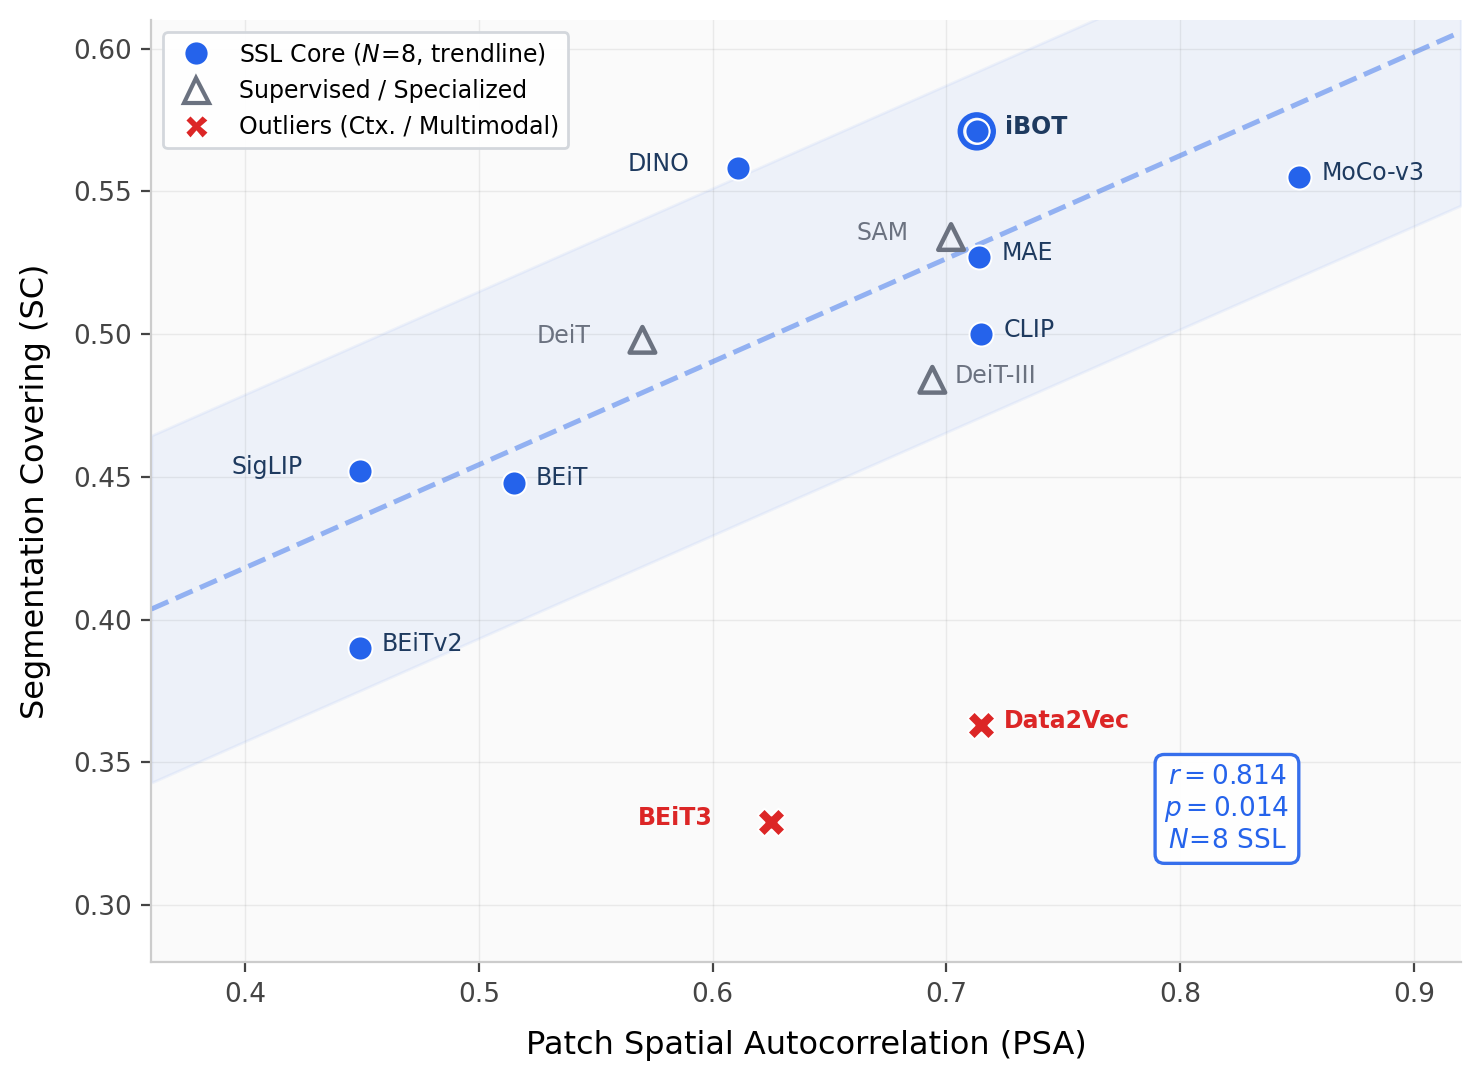
\includegraphics[width=0.72\textwidth]{fig_psa_sc_v2.png}
    \caption{PSA vs.\ SC for all 16 evaluated backbones. Blue circles: SSL core ($N=11$, trendline computed on this set, $r=0.861$, $p=0.0007$); gray triangles: supervised/specialized models (fit the trend but outside SSL scope); red crosses: mechanistic outliers (Data2Vec, BEiT3) that inflate PSA without semantic coherence.}
    \label{fig:psa_scatter}
    \vspace{-10pt}
\end{figure}

\subsection{Cross-Dataset Generalization}
\label{sec:boundary}

Having established PSA as a significant predictor on BSDS500, we ask whether this signal generalizes across annotation granularity.

\textbf{PSA generalizes to COCO and ADE20K.} PSA significantly predicts SC on COCO ($r=0.876$, $p=0.0004$, $N=11$) and ADE20K ($r=0.833$, $p=0.0015$, $N=11$). A metric computed on BSDS500 images predicts segmentation quality on datasets spanning boundary-level (BSDS500, avg.\ 19.6 regions), object-level (COCO, 80 categories), and scene-level (ADE20K, 150 categories) annotation granularity, as long as architecture is held constant.

\textbf{Why architecture control matters.} Earlier analysis using the mixed-architecture set found no PSA--SC correlation on COCO ($r = 0.12$). Mixing ViT-S/8 (patch size 8, 22M parameters) with ViT-B/16 (patch size 16, 86M parameters) introduces two confounds: patch size changes the spatial resolution of the feature grid (28$\times$28 vs.\ 14$\times$14 patches), directly affecting PSA values, while parameter count differences conflate capacity with pre-training paradigm. Controlling for architecture is essential when comparing representation-quality metrics across benchmarks.

\textbf{Backbone rankings reverse across tasks.} Table~\ref{tab:cross_dataset} shows that CLIP ranks last on BSDS500 (boundary task) but first on COCO (semantic task). No eigenspectral metric tracks this reversal---feature geometry is task-agnostic while segmentation quality is not. This is consistent with the alignment--uniformity framework \cite{wang2020alignment,tong2024eyes}: models with high semantic alignment (CLIP) excel at coarse object grouping but underperform where spatial feature smoothness matters.

\begin{table}[H]
\centering
\caption{SC across datasets for the mixed-architecture set. CLIP's ranking reversal (last on BSDS500, first on COCO) is not predicted by any eigenspectral metric.}
\label{tab:cross_dataset}
\small
\begin{tabular}{lccc}
\toprule
Backbone & BSDS500 & ADE20K & COCO \\
\midrule
DINO ViT-S/8     & \textbf{0.585} & \textbf{0.499} & 0.388 \\
MoCo-v3 ViT-B/16 & 0.555 & 0.487 & 0.381 \\
DINOv2 ViT-S/14  & 0.553 & 0.491 & 0.369 \\
iBOT ViT-S/16    & 0.549 & 0.495 & 0.382 \\
MAE ViT-B/16     & 0.527 & 0.429 & 0.387 \\
CLIP ViT-B/16    & 0.500 & 0.443 & \textbf{0.445} \\
\bottomrule
\end{tabular}
\vspace{-15pt}
\end{table}

\subsection{Boundary Conditions of PSA}
\label{sec:boundary_conditions}

For the eleven SSL backbones, PSA is a strong predictor ($r=0.862$, $p=0.0007$). To understand when this diagnostic fails, we evaluate five additional out-of-distribution models sharing the ViT-B/16 architecture (Fig.~\ref{fig:psa_scatter}).

\textbf{Supervised and segmentation-specialized models follow the spatial trend.} DeiT, DeiT-III, and SAM all lie close to the SSL trendline despite being trained with labels. These models are excluded from the core analysis as they violate the label-free premise, but their agreement with the trend further validates PSA as a genuine spatial property diagnostic.

\textbf{Contextualized and multimodal models mechanistically break PSA.} Data2Vec \cite{baevski2022data2vec} (PSA\,=\,0.715, SC\,=\,0.363) and BEiT3 \cite{wang2023beit3} (PSA\,=\,0.625, SC\,=\,0.329) exhibit high spatial smoothness but dramatically poor segmentation. Data2Vec regresses contextualized latent targets computed by an EMA teacher, forcing each patch to encode global scene context rather than local content. BEiT3 applies masked image modeling jointly with text, pulling patch features toward a shared image--language space. In both cases, neighboring patches become numerically similar---inflating PSA---but lose the dense, localized semantic boundaries required for unsupervised clustering. Extending to all 16 models drops the correlation ($r=0.581$, $p=0.037$): PSA remains significant overall but the outliers reduce predictive precision. PSA is a valid diagnostic specifically for SSL paradigms that preserve local spatial semantics.

\subsection{PSA Variants and Design Space}
\label{sec:psa_variants}

Is the 4-connected cosine formulation of PSA optimal, or merely one point in a design space? Table~\ref{tab:psa_variants} compares four variants on the $N=11$ SSL core set.

\begin{table}[H]
\centering
\caption{PSA variant ablation: Pearson $r$ with SC on BSDS500 ($N=11$ SSL core). All variants achieve significance; eigenvalue-weighted PSA achieves the strongest correlation.}
\label{tab:psa_variants}
\small
\begin{tabular}{lcc}
\toprule
Variant & $r$ & $p$ \\
\midrule
PSA (4-connected, cosine) & +0.864 & 0.0006 \\
PSA (8-connected, cosine) & +0.826 & 0.0018 \\
PSA (4-connected, neg.~$\ell_2$) & +0.818 & 0.0021 \\
\textbf{PSA-weighted} (eigenvalue-weighted cosine) & \textbf{+0.964} & \textbf{0.000002} \\
\bottomrule
\end{tabular}
\vspace{-10pt}
\end{table}

All four variants significantly predict SC, confirming that the spatial autocorrelation signal is robust to neighborhood definition and distance metric. The strongest variant---eigenvalue-weighted PSA, which weights each PCA dimension by its explained variance---achieves $r=0.964$ ($p<0.00001$), suggesting that dimensions carrying more variance contribute disproportionately to the spatial coherence signal. This is consistent with the top PCA components encoding large-scale semantic patterns that drive clustering quality. Incorporating eigenvalue weights further strengthens prediction, though this raises an open question about the interaction between spatial and spectral information---a direction for future work.

\subsection{PSA-Guided Backbone Selection}
\label{sec:psa_selection}

The practical value of PSA depends on whether it can guide backbone selection \emph{without labels}. We test this directly: rank all $N=11$ SSL backbones by PSA computed on BSDS500 images (no segmentation labels used), then evaluate their actual SC on ADE20K (a held-out dataset with different annotation granularity).

The PSA ranking on BSDS500 strongly predicts the actual SC ranking on ADE20K (Spearman $\rho=0.836$, $p=0.0013$; Pearson $r=0.824$, $p=0.0018$). The top-3 backbones by PSA (MoCo-v3, MAE, iBOT) are all in the actual top-5 by SC. Conversely, the bottom-3 by PSA (EVA-02, SigLIP, BEiTv2) are the actual bottom-3 by SC. A practitioner computing PSA on unlabeled images from any domain can reliably identify the best backbone for unsupervised segmentation without running a single evaluation.

\subsection{Spectral Complexity and Scene Difficulty: A Within-Backbone Analysis}
\label{sec:simpson}

Feature geometry metrics fail to predict SC across backbones (Sect.~\ref{sec:results}), but this could reflect pretraining paradigm differences rather than a general property of spectral complexity. A complementary question is: within a single backbone, do spectrally complex images segment worse? The answer is yes, and consistently so. Within each backbone, higher per-image spectral complexity significantly predicts \emph{worse} SC across multiple architectures (MAE: $r=-0.389$; DINO ViT-S/8: $r=-0.310$; iBOT: $r=-0.194$; DINOv2: $r=-0.185$; all significant at $p < 0.01$). CLIP shows a non-significant negative trend ($p=0.078$), with MoCo-v3 as the sole non-significant positive exception ($r=+0.079$, $p=0.267$; this does not persist on ADE20K, suggesting a dataset-specific artifact).

The two levels of analysis thus tell the same directional story but with different mechanisms. Across backbones, higher spectral richness is associated with lower SC because the pretraining objectives that create spectral diversity---sigmoid contrastive loss (SigLIP), masked tokenization (BEiT/BEiTv2)---happen to produce spatially incoherent features (low PSA). Within a backbone, a spectrally complex image is simply a complex scene, and complex scenes are harder to cluster regardless of backbone quality.

% ============================================================
% 5. CONCLUSION
% ============================================================
\section{Conclusion}

We demonstrated that eigenspectral and geometric metrics---despite their success in predicting classification performance---fundamentally fail to predict unsupervised segmentation quality. The critical property for dense pixel grouping is not geometric richness but feature-space spatial coherence: Patch Spatial Autocorrelation (PSA) emerges as a powerful, label-free diagnostic ($r=0.862$, $p=0.0007$, $N=11$) that generalizes across BSDS500, COCO, and ADE20K when architectural confounds are controlled. Eigenvalue-weighted PSA further strengthens prediction ($r=0.964$), and PSA-guided backbone selection without labels achieves Spearman $\rho=0.836$ agreement with ground-truth rankings on a held-out dataset. For backbone selection in dense prediction, the right question is not \emph{how spectrally diverse} the features are, but \emph{how spatially coherent} they are.

\textbf{Limitations.} The core SSL analysis spans $N=11$ ViT-B/16 backbones. Confounds include training data scale (SigLIP on WebLI-12B vs.\ CLIP on WIT-400M vs.\ OpenCLIP on LAION-2B) and the single architectural family (ViT-B/16). PSA breaks down for contextualized reconstruction (Data2Vec) and multimodal alignment (BEiT3) objectives. Future work should explore hierarchical spatial metrics, local CKA, or extend to convolutional and hybrid architectures.

% ============================================================
\begin{credits}
\vspace{-10pt}
\subsubsection{\discintname}
The authors have no competing interests to declare that are relevant to the content of this article.
\end{credits}

% ============================================================
% REFERENCES
% ============================================================
\begin{sloppypar}
\let\OLDthebibliography\thebibliography
\renewcommand\thebibliography[1]{
  \OLDthebibliography{#1}
  \setlength{\parskip}{0pt}
  \setlength{\itemsep}{0pt plus 0.3ex}
}
\begin{thebibliography}{32}
\bibitem{caron2021}
Caron, M., et al.: Emerging properties in self-supervised vision transformers. In: ICCV, pp.~9650--9660 (2021)
\bibitem{oquab2024}
Oquab, M., et al.: DINOv2: Learning robust visual features without supervision. TMLR (2024)
\bibitem{he2022}
He, K., et al.: Masked autoencoders are scalable vision learners. In: CVPR, pp.~16000--16009 (2022)
\bibitem{radford2021}
Radford, A., et al.: Learning transferable visual models from natural language supervision. In: ICML, pp.~8748--8763 (2021)
\bibitem{zhou2022ibot}
Zhou, J., et al.: iBOT: Image BERT pre-training with online tokenizer. In: ICLR (2022)
\bibitem{chen2021mocov3}
Chen, X., Xie, S., He, K.: An empirical study of training self-supervised vision transformers. In: ICCV, pp.~9640--9649 (2021)
\bibitem{hamilton2022}
Hamilton, M., et al.: Unsupervised semantic segmentation by distilling feature correspondences. In: ICLR (2022)
\bibitem{curie2025}
Curie, M., da Costa, P.: CLASP: Adaptive spectral clustering for unsupervised per-image segmentation. In: ICCV Workshops (2025)
\bibitem{wang2023lightweight}
Wang, X., et al.: A lightweight clustering framework for unsupervised semantic segmentation. arXiv:2311.18628 (2023)
\bibitem{melas2022}
Melas-Kyriazi, L., et al.: Deep spectral methods: A surprisingly strong baseline for unsupervised semantic segmentation. In: CVPR, pp.~8364--8373 (2022)
\bibitem{kim2024eagle}
Kim, S., et al.: EAGLE: Eigen aggregation learning for object-centric unsupervised semantic segmentation. In: CVPR (2024)
\bibitem{couairon2024diffcut}
Couairon, P., et al.: DiffCut: Catalyzing zero-shot semantic segmentation with diffusion features and recursive normalized cut. In: NeurIPS (2024)
\bibitem{garrido2023}
Garrido, Q., Balestriero, R., Lecun, Y., Bardes, A.: RankMe: Assessing the downstream performance of pretrained self-supervised representations by their rank. In: ICML, pp.~10929--10974 (2023)
\bibitem{agrawal2022}
Agrawal, T., et al.: $\alpha$-ReQ: Assessing representation quality in self-supervised learning by measuring eigenspectrum decay. In: NeurIPS, pp.~24892--24905 (2022)
\bibitem{tsitsulin2023}
Tsitsulin, A., et al.: Unsupervised universal embedding quality evaluation. arXiv:2307.1060 (2023)
\bibitem{ijcv2025ssl}
Pham, H., et al.: A closer look at benchmarking self-supervised pre-training with image classification. IJCV (2025)
\bibitem{amsaleg2018lid}
Amsaleg, L., et al.: Estimating local intrinsic dimensionality. In: KDD, pp.~29--38 (2015)
\bibitem{wang2020alignment}
Wang, T., Isola, P.: Understanding contrastive representation learning through alignment and uniformity on the hypersphere. In: ICML, pp.~9929--9939 (2020)
\bibitem{bardes2022vicreg}
Bardes, A., Ponce, J., LeCun, Y.: VICReg: Variance-invariance-covariance regularization for self-supervised learning. In: ICLR (2022)
\bibitem{tong2024eyes}
Tong, S., et al.: Eyes wide shut? Exploring the visual shortcomings of multimodal LLMs. In: CVPR (2024)
\bibitem{wysoczanska2024clipdinoiser}
Wysocza\'{n}ska, M., et al.: CLIP-DINOiser: Teaching CLIP a few DINO tricks for open-vocabulary semantic segmentation. In: ECCV (2024)
\bibitem{zhai2023siglip}
Zhai, X., et al.: Sigmoid loss for language image pre-training. In: ICCV, pp.~11975--11986 (2023)
\bibitem{amir2022}
Amir, S., et al.: Deep ViT features as dense visual descriptors. In: ECCVW (2022)
\bibitem{arbelaez2011}
Arbelaez, P., et al.: Contour detection and hierarchical image segmentation. IEEE TPAMI \textbf{33}(5), 898--916 (2011)
\bibitem{lin2014coco}
Lin, T.-Y., et al.: Microsoft COCO: Common objects in context. In: ECCV, pp.~740--755 (2014)
\bibitem{zhou2017ade20k}
Zhou, B., et al.: Scene parsing through ADE20K dataset. In: CVPR, pp.~633--641 (2017)
\bibitem{baevski2022data2vec}
Baevski, A., et al.: data2vec: A general framework for self-supervised learning in speech, vision and language. In: ICML, pp.~1298--1312 (2022)
\bibitem{wang2023beit3}
Wang, W., et al.: Image as a foreign language: BEiT pretraining for vision and vision-language tasks. In: CVPR, pp.~19175--19186 (2023)
\end{thebibliography}
\end{sloppypar}
\end{document}